\vspace{0.5cm}
\newline
\noindent \lecture{14}{25/11/2021}
\vspace{0.5cm}
\noindent Abbiamo visto che l'hamiltoniana di una \textit{Cooper Pair Box} risulta:
\begin{equation*}
    \hat H = E_C (\hat n - n_{g})^2 - E_J \cos{\hat \delta}
\end{equation*}
Per ora abbiamo usato la base del numero di particelle, ma generalmente si tende a studiare il sistema in una base diversa detta \textit{base di carica}.
Dopo aver definito $\ket j$ come autostato dato dal numero di quasiparticle in un elettrodo che soddisfa $\hat n \ket j = j \ket j$, possiamo proiettare l'hamiltoniana su una base di questi autostati:
\begin{equation*}
    \hat H = \sum_{ij} \ket{i}\bra{i}\hat H \ket{j}\bra{j}
\end{equation*}
Considerando solo il primo termine dell'hamiltoniana, potremo scrivere che:
\begin{equation*}
    \bra{j} \hat H \ket{j} = \bra{j}\hat n^2 \ket{j}-2n_g \bra{j}\hat n \ket{j} + n_g^2 \braket{j}{j} = j^2 - 2n_g j + n_g^2 = (j - n_g)^2
\end{equation*}
Dunque abbiamo, nella base della carica (i termini off-diagonal sono nulli):
\begin{equation*}
    \hat H =\sum_j E_C (j - n_g)^2\ket{j}\bra{j}
\end{equation*}
Vediamo ora cosa succede al coseno di $\delta$, il secondo termine dell'hamiltoniana originale.
Possiamo considerare l'identità di Eulero:
\begin{equation*}
    e^{i\delta} = 1 + i \delta - \frac{\delta^2}{2!}-i\frac{\delta^3}{3!} +\frac{\delta^4}{4!}+\cdots
\end{equation*}
Ricavando anche i commutatori\footnote{Si usano le relazioni $n=Q/2e$, $\Phi = \delta \hbar / 2e$, $[\Phi, Q] = i \hbar$}:
\begin{align*}
    \comm{\delta}{n} &= i \\
    \comm{e^{i\delta}}{n} &= -e^{i\delta}
\end{align*}
E troviamo che: $e^{\pm i \delta}\ket j = \ket{j\pm 1}$.
Infine troviamo la rappresentazione in base di carica del coseno di $\delta$:
\begin{equation*}
    \cos \delta = \sum_{ij} \ket i \bra i \cos \delta \ket j \bra j = \frac{1}{2}\sum_j \left(\ket{j+1}\bra{j}+ \ket{j}\bra{j+1}\right)
\end{equation*}
E gli operatori che compaiono nella formula appena scritta fondamentalmente spostano una quasiparticle dentro e fuori dall'isola.
Possiamo scrivere, dunque, l'hamiltoniana di una CPB nella base di carica:
\begin{equation*}
    \hat H = \underbrace{E_c\sum_j (j - n_g)^2 \ket{j} \bra {j}}_{E_1} - \underbrace{\frac{E_J}{2}\sum_j \left( \ket{j+1} \bra{j} +\ket{j}\bra{j+1} \right)}_{E_2}
\end{equation*}
Da questa espressione dell'hamiltoniana di una CPB possiamo scrivere, concentrandoci sui primi due livelli, in forma matriciale l'hamiltoniana del qubit corrispettivo\footnote{Stiamo approssimando, troncando lo sviluppo del coseno}.
\begin{align*}
    E_1 = E_C \begin{bmatrix}
     n_g^2 & 0 \\
     0 & (1-n_g)^2
    \end{bmatrix}
    &= E_C \begin{bmatrix}
     n_g^2 & 0 \\
     0 & 1-2n_g + n_g^2
    \end{bmatrix}\\
    &= E_C \begin{bmatrix}
     0 & 0 \\
     0 & 1 - 2n_g
    \end{bmatrix} + \cancel{E_C n_g^2\mathbb{I}}\\
    &= \frac{E_C}{2} \begin{bmatrix}
     -(1-2n_g) & 0 \\
     0 & 1-2n_g
    \end{bmatrix} + \cancel{\frac{E_c}{2}(1-2n_g)\mathbb I}
\end{align*}
L'idea è che abbiamo dei numeri $j$ collegati a variabili dinamiche e $n_g$ che è semplicemente una costante. Per questo posso andare a rimuovere i termini costanti.
Operando in ugual modo anche per il secondo termine, arriviamo a:
\begin{equation*}
    \hat H =-\frac{E_C}{2}(1-2n_g)\hat \sigma_z - \frac{E_J}{2}\hat \sigma_x
\end{equation*}
Questa espressione è una forma particolare della più generale hamiltoniana per un qubit (indicata con pedice due perché relativa a un sistema a due livelli):
\begin{equation*}
    \hat H_2 = -\frac{1}{2}\left(\varepsilon \sigma_z + \Delta \sigma_x \right)
\end{equation*}
dove, in questo caso:
\begin{equation*}
    \varepsilon = E_C(1-2n_g)
\end{equation*}
\begin{equation*}
    \Delta = E_J
\end{equation*}
\begin{equation*}
    n_g=\frac{1}{2} \rightarrow \varepsilon=0
\end{equation*}
Inoltre possiamo identificare il caso in cui $n_g = \frac{1}{2}$ che implica $\varepsilon=0$.
Ora non abbiamo più, però, un'hamiltoniana diagonale (perché abbiamo cambiato base). Dobbiamo quindi cercare nuovamente gli autovalori di H e i rispettivi autostati.
Abbiamo:
\begin{equation*}
    \hat H=-\frac{1}{2}\begin{pmatrix} \varepsilon & \Delta \\ \Delta & -\varepsilon \end{pmatrix}
\end{equation*}
E, risolvendo, otteniamo gli autovalori per l'hamiltoniana approssimata:
\begin{equation*}
    E_{1,2}=\pm \frac 12 \sqrt{\varepsilon^2 + \Delta^2} = \pm \frac 12 \sqrt{E_c^2 (1-2n_g)^2 + E_J^2}
\end{equation*}
E i rispettivi autovettori (espressi nella base computazionale):
\begin{align*}
    \ket{E_1} = \frac{1}{\sqrt{2}}(\ket{0} + \ket{1})\\
    \ket{E_2} = \frac{1}{\sqrt{2}}(\ket{0} - \ket{1})
\end{align*}

\begin{figure}[!htp]
    \centering
    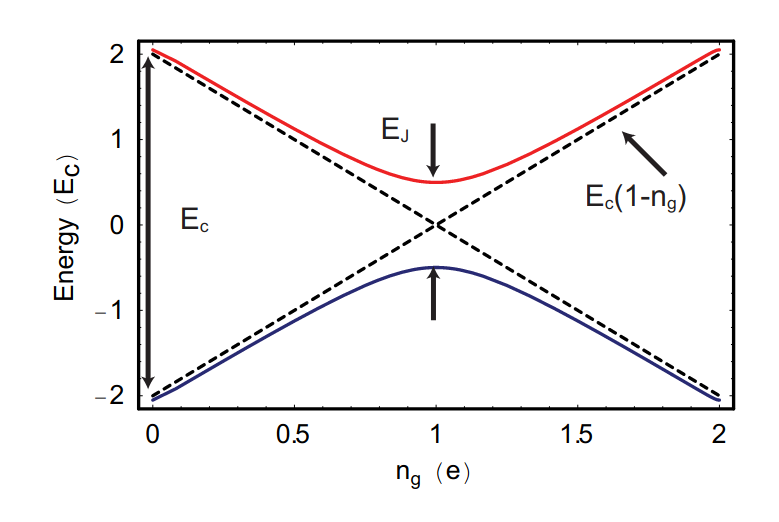
\includegraphics[width=0.7\textwidth]{images/CPB_ng_vs_ec.png}
    \caption{\url{https://rsl.yale.edu/sites/default/files/files/RSL_Theses/SchusterThesis.pdf}}
\end{figure}
\noindent In realtà, benché abbiamo visto solo un caso specifico, le hamiltoniane di tutti i qubit possono essere scritte in funzione di $\sigma_x$ e $\sigma_z$.
Talvolta può essere utile lavorare in un sistema ruotato di $\theta_m$, dove $\theta_m$ è l'angolo fra il coefficienti di $\sigma_z$ e $\sigma_x$.
\begin{equation*}
    \tan \theta_m = \frac{E_j}{E_c(1-2n_g)} 
\end{equation*}
In questo modo abbiamo un'hamiltoniana più semplice:
\begin{equation*}
    \hat H = - \frac{\hbar}{2}\omega_q \hat \sigma_z
\end{equation*}
con $\omega_q = \sqrt{E_j^2 + E_c^2 (1-2n_g)^2}$
\subsection{Limite TRANSMON}
Studiamo ora il limite per cui $E_C \ll E_J$. Questa tipologia di \textbf{charge qubit} prende il nome, in questo limite, di TRANSMON.
Questo limite è particolarmente interessante perché i livelli energetici perdono quasi del tutto la  dipendenza dal numero di quasiparticle nell'isola (la differenza fra due picchi va come $e^{-\sqrt{8E_J/E_C}}$). Ciò consente di avere un'energia di transizione ben definita che è necessaria per controllare il qubit. 
Il problema che sorge, tuttavia, riguarda l'anarmonicità fra i livelli che decresce. Possiamo dunque dire che un alto rapporto $E_J/E_C$ sia conveniente? Per studiarlo dobbiamo tornare a studiare l'hamiltoniana (ma scopriremo che l'anarmonicità è sufficiente).
A meno di termini costanti potremo scrivere (espandendo il coseno ($-E_J \cos \delta = - E_J + \frac{E_J \delta^2}{2} - \frac{E_J \delta^4}{24}+ \cdots$):
\begin{equation*}
    \hat H = \frac{Q^2}{2C}-E_J+ \frac{E_J}{2}\delta^2- \frac{E_J }{24}\delta^4 
    =\frac{Q^2}{2C}+\frac{\Phi^2}{2L_J}-\frac{\Phi^4}{24L_J \Phi^2_0} - E_J
\end{equation*}
Dove abbiamo utilizzato le relazioni $\delta=\Phi/\Phi_0$ e $E_J=\Phi^2_0/L_J$. Considerando anche che:
\begin{align*}
    \hat \Phi=\sqrt{\frac{\hbar \sqrt{\frac{L}{C}}}{2}}(\hat a+\hat a^\dagger) \\
    \hat Q=-i\sqrt{\frac{\hbar}{2\sqrt{\frac{L}{C}}}}(\hat a-\hat a^\dagger)
\end{align*}
possiamo riscrivere $\hat H$ come (di nuovo rimuovo i termini costanti):
\begin{equation*}
    \hat H = \hbar \omega_J \hat a^\dagger \hat a - \frac{E_C}{12}(\hat a+\hat a^\dagger)^4
\end{equation*}
dove abbiamo:
\begin{equation*}
    \omega_J = \sqrt{\frac{1}{L_J C}}= \frac{\sqrt{8E_J E_C}}{\hbar}
\end{equation*}
Questa non è propriamente la frequenza di risonanza del qubit (che è definita come la differenza di energia fra i primi due livelli energetici) perché il secondo termine di $\hat H$ contribuisce con alcuni addendi $\hat a$ e $\hat a^\dagger$. Considerando solo questi (i termini che non hanno $\hat a$ e $\hat a^\dagger$ bilanciati vengono rimossi nella \textit{rotating wave approximation} con $\omega_J$) e il commutatore $\comm{\hat a}{\hat a^\dagger}=1$,  posso scrivere l'hamiltoniana:
\begin{equation*}
     \hat H = \left(\sqrt{8 E_J E_C} - E_C \right) \hat a^\dagger \hat a - \frac{E_C}{2} \hat a^\dagger \hat a (\hat a^\dagger \hat a - 1)
\end{equation*}
Questa è l'hamiltoniana approssimata di un qubit TRANSMON che ha frequenza di risonanza:
\begin{equation*}
    \omega_q = \frac{\sqrt{8E_J E_C} - E_C}{\hbar} = \omega_J - \frac{E_C}{\hbar}
\end{equation*}
E anarmonicità:
\begin{equation*}
    \alpha = -\frac{E_C}{\hbar}
\end{equation*}
\subsubsection{Realizzazione fisica di un TRANSMON}
Diamo qualche numero reale relativo a questo tipo di qubit (che è quello maggiormente utilizzato oggi).
Tendenzialmente si utilizza un regime $E_J = 50E_C$. 
Una giunzione Josephson è molto piccola con dimensioni nell'ordine del micrometro e, ad essa, corrisponde una capacità dell'ordine del $\sim \text{fF}$. Il comune design attuale dei TRANSMON è il cosidetto XMON. Due elettrodi incrociati occupano la maggior parte dello spazio e sono connessi ai sistemi di lettura e controllo, al lato estremo di uno di questi elettrodi sono poste due giunzioni Josephson col qubit vero e proprio.
\begin{figure}[!htp]
    \centering
    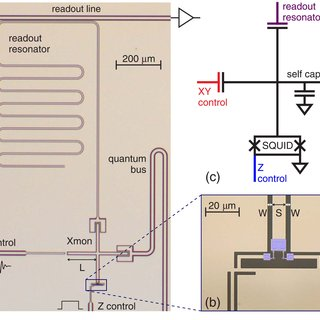
\includegraphics[width=0.7\textwidth]{images/xmon_qubit.jpg}
    \caption{\url{https://www.researchgate.net/publication/342301953_Superconducting_Quantum_Computing_A_Review}}
\end{figure}
La capacità principale (data dai due grandi elettrodi) aggiunge $10-100\text{ pF}$. Mentre la giunzione porta $\sim10 \text{ nH}$ (devo calibrare il circuito con cautela in modo da avere anche frequenze accessibili). Tutto ciò porta a una corrente critica di $I_0=0.03\, \mu \text{A}$.
Questo, in realtà, è il parametro principale che controlla la frequenza del qubit. La teoria (non studiata da noi) ci porta a scrivere una relazione esatta fra $I_0$, $T$ e $\omega_q$; perciò anche a temperatura ambiente potremmo studiare la frequenza di risonanza.
Coi numeri appena scritti si arriva a: $\omega\sim 30 \text{ GHz}$ e anarmonicità di $f\sim \text{ MHz}$.
Queste analisi possono essere svolte a livello di simulazioni altamente precise.